\chapter{A Tractable Bound on Approximating Kemeny Aggregation}
\label{chap:kemeny}

\begin{chapabstract}{Abstract:}
Due to its numerous applications, rank aggregation has become a problem of major interest across many fields of the computer science literature. In the vast majority of situations, Kemeny consensus is considered as the ``golden'' solution. It is however well known that its computation is NP-hard. Much contribution have thus been devoted to establishing various results to apprehend this complexity. In this chapter, we introduce a practical method to predict, given a dataset and a ranking typically output by some approximate procedure, how close this ranking is to the Kemeny consensus of the dataset. A major strength of the proposed method is its generality: it requires little assumption on the dataset nor the ranking. Furthermore, it relies on a geometric interpretation of Kemeny aggregation that we believe could paves way to other results beyond those presented in this chapter. This study has been published as joint work with Anna Korba and Eric Sibony \cite{Jiao2016Controlling}.
\end{chapabstract}
\vskip 0.2in
\begin{chapabstract}{R�sum� :}
En raison de ses nombreuses applications, l'agr�gation de classements est devenue un probl�me d'int�r�t majeur dans de nombreux domaines de la litt�rature en science informatique. Dans la grande majorit� des situations, le consensus de Kemeny est consid�r� comme la solution <<dor�e>>. Il est cependant bien connu que son calcul est NP-difficile. Par cons�quent, de nombreuses contributions ont �t� consacr�es � l'�tablissement de divers r�sultats pour appr�hender cette complexit�. Dans ce chapitre, nous introduisons une m�thode pratique pour pr�dire, compte tenu d'un ensemble de donn�es et d'un classement g�n�ralement produit par une proc�dure approximative, quelle est la proximit� de ce classement au consensus de Kemeny sur l'ensemble de donn�es. Une force majeur de la m�thode propos�e est sa g�n�ralit� : elle n�cessite peu d'hypoth�ses sur l'ensemble de donn�es, ni sur le classement. En outre, il repose sur une interpr�tation g�om�trique de l'agr�gation de Kemeny que nous croyons pouvoir ouvrir la voie � d'autres r�sultats au-del� de ceux pr�sent�s dans ce chapitre. Cette �tude a �t� publi�e en collaboration avec Anna Korba et Eric Sibony \cite{Jiao2016Controlling}.
\end{chapabstract}

\section{Introduction}

Given a collection of rankings on a set of alternatives, how to aggregate them into one ranking? This rank aggregation problem has gained a major interest across many research fields. Starting from elections in social choice theory \cite{Borda1781Memoire, Condorcet1785Essai, Arrow1950difficulty, Xia2015Generalized}, it has been applied to meta-search engines \cite{Dwork2001Rank, Renda2003Web, Desarkar2016Preference}, competitions ranking \cite{Davenport2005Ranking, Deng2014Bayesian}, analysis of biological data \cite{Kolde2012Robust, Patel2013Hierarchical} or natural language processing \cite{Li2014Learning, Zamani2014Regression} among others.

Among many ways of formulating the problem of rank aggregation stands out the Kemeny aggregation \cite{Kemeny1959Mathematics}. Defined as the problem of minimizing a cost function over the symmetric group (see Section \ref{secA:problem-statement} for definition), its solutions, called Kemeny consensuses, have been shown to satisfy desirable properties from many points of view \cite{Young1978consistent}.

Computing a Kemeny consensus is however NP-hard, even for only four rankings \cite{Bartholdi1989computational, Cohen1999Learning, Dwork2001Rank}. This fact has motivated the research community to introduce many approximate procedures and to evaluate them on datasets (see, for instance, \cite{Schalekamp2009Rank, Ali2012Experiments}). It has also triggered a tremendous amount of work of obtaining theoretical guarantees on these procedures and more generally in understanding the complexity of Kemeny aggregation from various perspectives. Some have proven bounds on the approximation cost of the approximate procedures \cite{Diaconis1977Spearmans, Coppersmith2006Ordering, VanZuylen2007Deterministic, Ailon2008Aggregating, Freund2015Rank}, while some have established recovery properties \cite{Saari2000geometric, Procaccia2012Maximum}. Notably it has been shown that exact Kemeny aggregation is tractable if some quantity is known on the dataset \cite{Betzler2008Fixed, Betzler2009How, Cornaz2013Kemeny} or if the dataset satisfies some conditions \cite{Brandt2015Bypassing}. Besides, some contributions have established approximation bounds that can be computed on the dataset \cite{Davenport2004computational, Conitzer2006Improved, Sibony2014Borda}.

In this chapter we introduce a novel approach to apprehend the complexity of Kemeny aggregation. Consider the following question: \textit{Given a dataset and a ranking typically output by some approximate procedure, can we predict how close the ranking is to any Kemeny consensus without computing the latter?} We exhibit a tractable quantity that allows to give a positive answer to this question. The main contribution of our results is a simple and practical method to obtain such a guarantee for the outcome of an aggregation procedure on any dataset. A major strength of our approach is its generality: it applies to all aggregation procedures and to any dataset. Further, our results are based on a geometric analysis of Kemeny aggregation (see Section \ref{secA:geometry}) that has been unprecedentedly exploited in the literature yet but constitutes a powerful tool. We thus take efforts to explain it in details. We believe that it could pave way to many other results on Kemeny aggregation beyond those presented here.

The chapter is structured as follows. Section \ref{secA:problem-statement} introduces the general notations and states the question of interest. The geometric analysis is detailed in Section \ref{secA:geometry} and further studied in Section \ref{secA:proof} while our main result is presented in Section \ref{secA:main-result}. Finally, numerical experiments are reported in Section \ref{secA:experiments} to address the efficacy and usefulness of our method on datasets from real-world applications.



\section{Kemeny Aggregation Problem}
\label{secA:problem-statement}


Let $\n = \cbr{1,\dots,n}$ be a set of alternatives to be ranked. In this study, we focus only on total rankings. A total ranking $a_1 \succ \dots \succ a_n$ on $\n$ is interchangeably seen as the permutation $\sigma$ of $\n$ that maps an item to its rank: $\sigma(a_i)=i$ for $i \in \n$. The set of all permutations of $\n$ is called the symmetric group and denoted by $\Sn$. Given a collection of $N$ permutations $\DN = \left(\sigma_{1},\dots,\sigma_{N}\right)\in\Sn^{N}$, Kemeny aggregation aims at solving
\begin{equation}
\label{eqA:Kemeny-aggregation}
\min_{\sigma\in\Sn} \sum_{t=1}^{N}d(\sigma,\sigma_{t}) \,,
\end{equation}
where $d$ is the Kendall's tau distance defined for $\sigma,\sigma' \in \Sn$ as the number of their pairwise disagreements: $d(\sigma,\sigma') = \sum_{1\leq i < j \leq n}\hollowone\{(\sigma(j)-\sigma(i))(\sigma'(j)-\sigma'(i))<0\}$. The objective function in \eqref{eqA:Kemeny-aggregation} denotes the cost, and a permutation $\sigstar$ solving \eqref{eqA:Kemeny-aggregation} is called a Kemeny consensus. We denote by $\KN$ the set of Kemeny consensuses on the dataset $\DN$.

Exact Kemeny aggregation is NP-hard: it cannot be solved efficiently with a general procedure. This does not mean however that nothing can be done. For example, it is clear that on a dataset where all permutations are equal to a $\sigma_{0}\in\Sn$, the Kemeny consensus is trivially given by $\sigma_{0}$. Many contributions from the literature have thus focused on particular approaches to apprehending some part of the complexity of Kemeny aggregation. The examples given in the introduction generally fall in three categories:
\begin{bulletList}
	\item \textbf{General guarantees for approximate procedures.} These results provide a bound on the cost of a specific voting rule, valid for any dataset \cite{Diaconis1977Spearmans, Coppersmith2006Ordering, VanZuylen2007Deterministic, Ailon2008Aggregating, Freund2015Rank}.
	\item \textbf{Bounds on the approximation cost computed from the dataset.} These results provide a bound, either on the cost of a consensus or on the cost of the outcome of a specific voting rule, that depends on a quantity computed from the dataset \cite{Davenport2004computational, Conitzer2006Improved, Sibony2014Borda}.
	\item \textbf{Conditions for the exact Kemeny aggregation to become tractable.} These results ensure the tractability of exact computation of Kemeny aggregation if the dataset satisfies some condition or if some quantity is known from the dataset \cite{Betzler2008Fixed, Betzler2009How, Cornaz2013Kemeny, Brandt2015Bypassing}.
\end{bulletList}
In this chapter, we introduce a novel approach, which falls into the second category above, to apprehend the complexity of Kemeny aggregation by considering the following question (henceforth referred to as The Question):

\begin{question*}
Let $\sigma\in\Sn$ be a permutation, typically output by a computationally efficient aggregation procedure on $\DN$. Can we use tractable quantities to give an upper bound on the distance $d(\sigma,\sigstar)$ between $\sigma$ and any Kemeny consensus $\sigstar$ on $\DN$?
\end{question*}


The answer to The Question is positive as we will elaborate in this study. We propose an upper bound, guaranteed by Theorem \ref{thmA:method}, that reads: for any $\sigma$ and $\DN$, we have $d(\sigma,\sigstar)\leq \kmin$ for all consensuses $\sigstar\in\KN$, where $\kmin$ is defined in \eqref{eqA:k-min}. We would like to stress a major strength of our method compared to those previously studied in literature that is the generality: it can be applied to any dataset $\DN$ and any permutation $\sigma$ with little assumption on neither. This is because it exploits a powerful geometric framework for the analysis of Kemeny aggregation.



\section{Geometric Analysis of Kemeny Aggregation}
\label{secA:geometry}

Because of its rich mathematical structure, Kemeny aggregation can be analyzed from many different point of views. For instance, some contributions deal directly with the combinatorics of the symmetric group \cite{Diaconis1977Spearmans, Blin2011Median}, some work on the pairwise comparison graph \cite{Coppersmith2006Ordering, Conitzer2006Improved, Jiang2011Statistical}, and some exploit the geometry of the Permutahedron \cite{Saari2000geometric}. In this chapter, we analyze it via the Kendall embedding \cite[Theorem 1]{Jiao2015Kendall}. For the self-containment of this chapter, recall from the proof of Theorem \ref{thm2:main} that we have used the following definition.\footnote{We will omit the scaling constant $\frac{1}{\binom{n}{2}}$ due to its irrelevance in this study and use $\phi$ instead of $\Phi$ to distinguish this trivial difference.}

\begin{definition}[Kendall embedding]
The Kendall embedding is the mapping $\phi : \Sn \rightarrow \RR^{\binom{n}{2}}$ defined by
\[
\phi:\sigma \mapsto 
\left(\begin{array}{c}
\vdots\\
\sgn(\sigma(i)-\sigma(j))\\
\vdots
\end{array}\right)_{1 \leq i < j \leq n} \,,
\]
where the sign function $\sgn(x) = 1$ if $x > 0$ and $-1$ if $x < 0$ and $0$ otherwise.
\end{definition}

The Kendall embedding $\phi$ maps a permutation to a vector in $\RR^{\binom{n}{2}}$ where each coordinate is indexed by an (unordered) pair $\{i,j\}\subset\n$ (we choose $i<j$ by convention). Though this vector representation is equivalent to representing a permutation as a flow on the complete graph on $\n$, it allows us to perform a geometric analysis of Kemeny aggregation in the Euclidean space $\RR^{\binom{n}{2}}$. Denoting by $\innerprod{\cdot,\cdot}$ the canonical inner product and $\nm{\cdot}$ the Euclidean norm, the starting point of our analysis is the following result, already brought up by \cite{Barthelemy1981median} and rephrased in the proof of Theorem \ref{thm2:main}.

\begin{proposition}[Background results]
\label{propA:background-result}
For all $\sigma,\sigma'\in\Sn$,
\[
\nm{\phi(\sigma)} = \sqrt{\frac{n(n-1)}{2}} := R \;\text{and}\; \nm{\phi(\sigma) - \phi(\sigma')}^2 = 4 d(\sigma,\sigma') \,,
\]
and for any dataset $\DN=(\sigma_{1},\dots\sigma_{N})\in\Sn^{N}$, Kemeny aggregation \eqref{eqA:Kemeny-aggregation} is equivalent to the minimization problem
\begin{equation}
\label{eqA:reformulation}
\min_{\sigma\in\Sn} C_{N}(\sigma) := \Vert\phi(\sigma)-\phi(\DN)\Vert^{2} \,,
\end{equation}
where
\begin{equation}
\label{eqA:mean-embedding}
\phi\br{\DN} := \frac{1}{N}\sum_{t=1}^{N}\phi\br{\sigma_t}.
\end{equation}
\end{proposition}

Proposition \ref{propA:background-result} leads to the following geometric point of view of Kemeny aggregation, illustrated by Figure \ref{figA:geometric-interpretation}. First, as $\nm{\phi(\sigma)} = \sqrt{n(n-1)/2}$ for all $\sigma\in\Sn$, the embeddings of all the permutations in $\Sn$ lie on a sphere centered at $0$ with radius $R = \sqrt{n(n-1)/2}$. Notice that $\nm{\phi(\sigma) - \phi(\sigma')}^2 = 4 d(\sigma,\sigma')$ for all $\sigma,\sigma'\in\Sn$ implies that $\phi$ is injective, in other words that it maps two different permutations to two different points on the sphere. A dataset $\DN = (\sigma_{1},\dots,\sigma_{N})\in\Sn^{N}$ is thus mapped to a weighted point cloud on this sphere, where for any $\sigma\in\Sn$, the weight of $\phi(\sigma)$ is the number of times $\sigma$ appears in $\DN$. The vector $\phi(\DN)$, defined by \eqref{eqA:mean-embedding}, is then equal to the barycenter of this weighted point cloud. We call it the \textit{mean embedding} of $\DN$. Now, the reformulation of Kemeny aggregation given by \eqref{eqA:reformulation} means that a Kemeny consensus is a permutation $\sigstar$ whose embedding $\phi(\sigstar)$ is closest to $\phi(\DN)$, \textit{with respect} to the Euclidean norm in $\RR^{\binom{n}{2}}$.

\begin{figure}[!htbp]
	\begin{center} 
		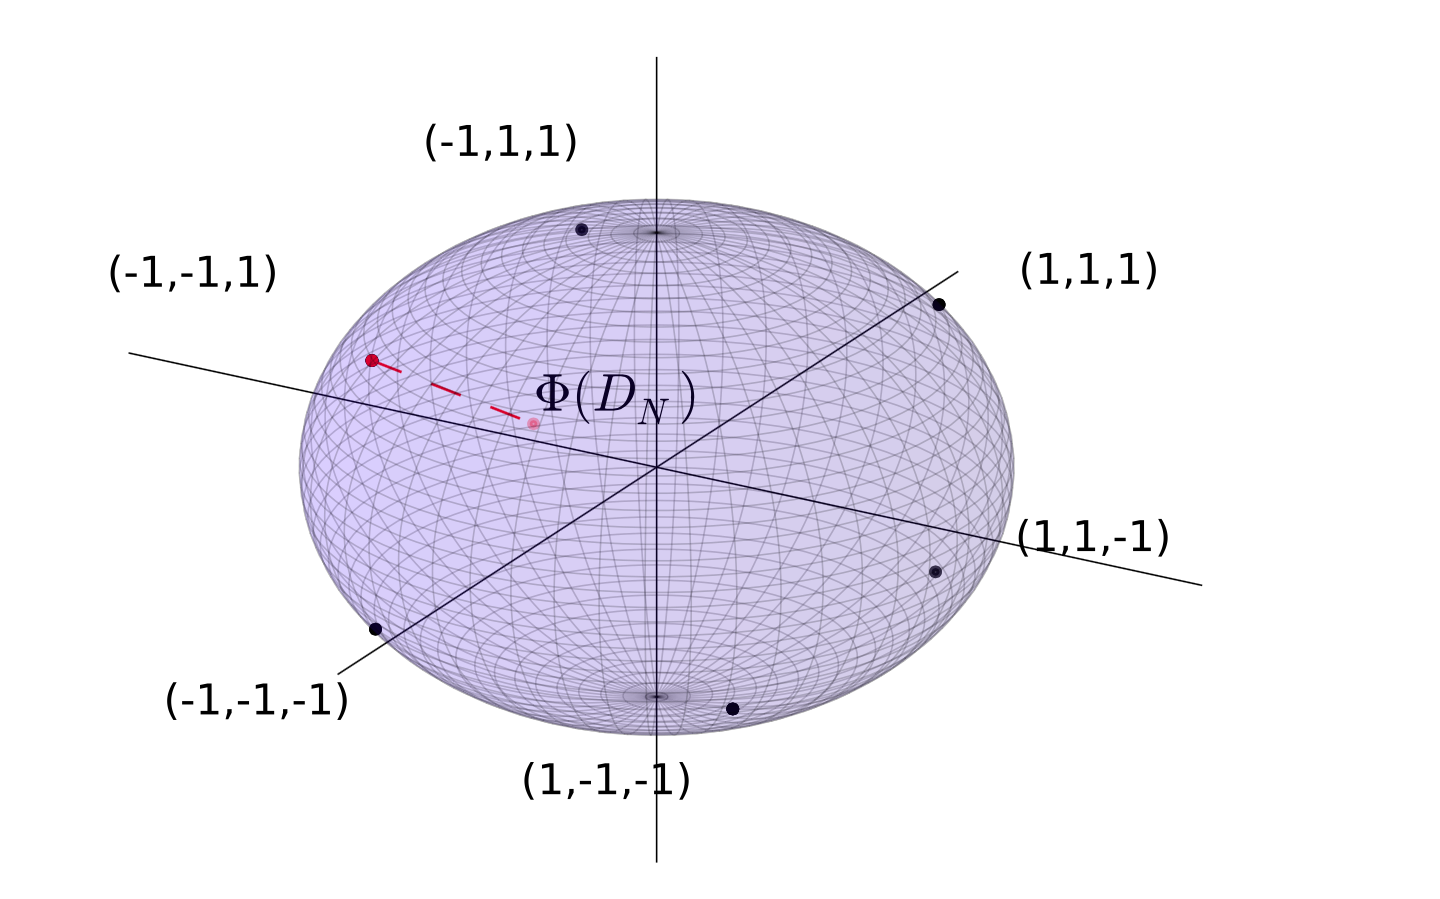
\includegraphics[trim=2cm 2cm 3cm 2cm, clip=true, width=0.6\textwidth, height=2.5in]{ch-kemeny/figures/3d1test}
	\end{center}
	\caption{Kemeny aggregation for $n=3$.}
	\label{figA:geometric-interpretation}
\end{figure}


From an algorithmic point of view, Proposition \ref{propA:background-result} naturally decomposes problem \eqref{eqA:Kemeny-aggregation} of Kemeny aggregation in two steps: first compute the mean embedding $\phi(\DN)$ in the space $\RR^{\binom{n}{2}}$, and then find a consensus $\sigstar$ as a solution of problem \eqref{eqA:reformulation}. The first step is naturally performed in $O(Nn^{2})$ operations. The NP-hardness of Kemeny aggregation thus stems from the second step. In this regard, one may argue that having $\phi(\DN)$ does not greatly alleviate the complexity in identifying an exact Kemeny consensus. However, a closer look at the problem leads us to asserting that $\phi(\DN)$ contains rich information about the location of the Kemeny consensuses. More specifically, we show in Theorem \ref{thmA:method} that the knowledge of $\phi(\DN)$ helps to provide an upper bound for the distance between a given permutation $\sigma\in\Sn$ and any Kemeny consensus $\sigstar$.


In fact, Proposition \ref{propA:background-result} implies that Kemeny's rule is a ``Mean Proximity Rule'', a family of voting rules introduced in \cite{Zwicker2008Consistency} and further studied in \cite{Lahaie2014Neutrality}. Our approach actually applies more generally to other voting rules from this class but we focus our discussion on Kemeny's rule in this study for the sake of clarity.


\section{Controlling the Distance to Kemeny Consensus}
\label{secA:main-result}

In this section, we now state our main results and demonstrate with an illustrative example how our proposed method addresses The Question. For a permutation $\sigma\in\Sn$, let us define the angle $\theta_{N}(\sigma)$ between $\phi(\sigma)$ and $\phi(\DN)$ by 
\begin{equation}
\label{eqA:cosinus}
\cos(\theta_{N}(\sigma)) = \frac{\innerprod{\phi(\sigma),\phi(\DN)}}{{\nm{\phi(\sigma)}\nm{\phi(\DN)}}},
\end{equation}
with $0 \leq \theta_{N}(\sigma)\leq \pi$ by convention.

\begin{thm}
\label{thmA:method}
Let $\DN\in\Sn^N$ be a dataset and $\sigma\in\Sn$ a permutation. For any integer $0 \leq k \leq \binom{n}{2}-1$, one has the following implication:
\[
\cos(\theta_{N}(\sigma)) > \sqrt{1-\frac{k+1}{\binom{n}{2}}}\quad\Longrightarrow\quad \max_{\sigstar\in\KN}d(\sigma,\sigstar) \leq k.
\]
\end{thm}

The proof of Theorem \ref{thmA:method} along with its geometric interpretation are postponed to Section \ref{secA:proof}. Broadly speaking, Theorem \ref{thmA:method} ensures that if the angle $\theta_{N}(\sigma)$ between the embedding $\phi(\sigma)$ of a permutation $\sigma\in\Sn$ and the mean embedding $\phi(\DN)$ is small, then the Kemeny consensuses cannot be too far from $\sigma$. Its application in practice is straightforward. Assume that one applies an aggregation procedure on $\DN$, say the Borda Count for instance, that outputs $\sigma$. A natural question is then: how far is it from the Kemeny consensuses in terms of Kendall's tau distance? It is well known that the Kendall's tau distance takes values in $\{0,\dots,\binom{n}{2}\}$ \cite{Stanley1986Enumerative}. Consequently, the distance is at most equal to $\max_{\sigma',\sigma''\in\Sn} d(\sigma',\sigma'') = \binom{n}{2}$. But if one computes the quantity $\cos(\theta_{N}(\sigma))$, a better bound can be allowed due to Theorem \ref{thmA:method}. More specifically, the best bound is given by the minimal $k\in\{0,\dots,\binom{n}{2}-1\}$ such that $\cos(\theta_{N}(\sigma)) > \sqrt{1-(k+1)/\binom{n}{2}}$. Denoting by $\kmin(\sigma;\DN)$ this integer, it is easy to see that
\begin{equation}
\label{eqA:k-min}
\kmin(\sigma;\DN) = 
\left\{
\begin{array}{ll}
\left\lfloor \binom{n}{2}\sin^{2}(\theta_{N}(\sigma))\right\rfloor & \text{if } 0 \leq \theta_{N}(\sigma) \leq \frac{\pi}{2}\\
\binom{n}{2} & \text{if } \frac{\pi}{2} \leq \theta_{N}(\sigma) \leq \pi.
\end{array}
\right.
\end{equation}
where $\lfloor x\rfloor$ denotes the integer part of the real $x$. We formalize this method (henceforth referred to as The Method) in the following description.

\begin{method*}
Let $\DN\in\Sn^{N}$ be a dataset and let $\sigma\in\Sn$ be a permutation considered as an approximation of Kemeny's rule. In practice $\sigma$ is the consensus returned by a tractable voting rule. Then by Theorem \ref{thmA:method}, we have $d(\sigma,\sigstar) \leq \kmin(\sigma;\DN)$ for any Kemeny consenus $\sigstar\in\KN$, where $\kmin(\sigma;\DN)$ is obtained by \eqref{eqA:k-min}.
\end{method*}

The following proposition ensures that The Method has tractable complexity.

\begin{proposition}[Complexity of The Method]
The application of The Method has complexity in time $O(Nn^{2})$.
\end{proposition}

With a concrete example, we demonstrate the applicability and the generality of The Method.

\begin{example}[Application of The Method to the sushi dataset]
We report here the results of a case-study on the sushi dataset provided by \cite{Kamishima2003Nantonac} to illustrate our method. The dataset consists of $N=5000$ total rankings given by different individuals of the preference order on $n=10$ sushi dishes such that a brute-force search for the Kemeny consensus is already very computationally intensive. To apply our method, we selected seven tractable voting rules, denoted by $\sigma$, as approximate candidates to Kemeny's rule to provide an initial guess (details of voting rules can be found in Section \ref{secA:votingrules}). Table \ref{tabA:sushi} summarizes the values of $\cos(\theta_N(\sigma))$ and $\kmin(\sigma)$, respectively given by \eqref{eqA:cosinus} and \eqref{eqA:k-min}. Results show that on this particular dataset, if we use for instance Borda Count to approximate a Kemeny consensus, we are confident that any exact consensus has a distance of at most 14 to the approximate ranking. We detail empirical analysis of the results further in Section \ref{secA:experiments}.
\end{example}

\begin{table}[!htbp]
	\caption{Summary of a case-study on the applicability of The Method with the sushi dataset $(N=5000,n=10)$. Rows are ordered by increasing $\kmin$ (or decreasing cosine) value.}
	\label{tabA:sushi}
	\begin{center}
		\begin{tabular}{c|c|c}
			\hline
			Voting rule & $\cos(\theta_N(\sigma))$ & $\kmin(\sigma)$ \\
			\hline
			Borda & 0.820 & 14 \\
			Copeland & 0.822 & 14 \\
			QuickSort & 0.822 & 14 \\
			Plackett-Luce & 0.80 & 15 \\
			2-approval & 0.745 & 20 \\
			1-approval & 0.710 & 22 \\
			Pick-a-Perm & 0.383$^\dag$ & 34.85$^\dag$ \\
			Pick-a-Random & 0.377$^\dag$ & 35.09$^\dag$ \\
			\hline		
		\end{tabular}
	\end{center}
	\rule{0in}{1.2em}$^\dag$\scriptsize  For randomized methods such as Pick-a-Perm and Pick-a-Random, results are averaged over 10,000 computations.
\end{table}



\section{Geometric Interpretation Revisit and Proof of Theorem \ref{thmA:method}}
\label{secA:proof}

This section details the proof of Theorem \ref{thmA:method} based the geometric interpretation introduced in Section \ref{secA:geometry}. We deem that our proof has indeed a standalone interest, and that it could pave way to other profound results on Kemeny aggregation.

\subsection{Extended Cost Function}

Recall that the Kemeny consensuses of a dataset $\DN$ are the solutions of the problem \eqref{eqA:reformulation}:
\[
\min_{\sigma\in\Sn}C_{N}(\sigma) = \nm{\phi(\sigma)-\phi(\DN)}^{2} \,.
\]
This is an optimization problem on the discrete set $\Sn$, naturally hard to analyze. In particular the shape of the cost function $C_{N}$ is not easy to understand. However, since all the vectors $\phi(\sigma)$ for $\sigma\in\Sn$ lie on the sphere
\[
\Sphere := \left\{ x \in \RR^{\binom{n}{2}} \vert \nm{x} = R \right\} \,,
\]
where radius $R$ is the equal norm of the embedded point of any permutation and by Proposition \ref{propA:background-result},
\[
R = \sqrt{\frac{n(n-1)}{2}} \,.
\]
It is natural to consider the relaxed problem on $\Sphere$ that reads
\[
\min_{x\in\Sphere}\CN(x):=\nm{x-\phi(\DN)}^{2} \,.
\]
We call $\CN$ the extended cost function with domain $\Sphere$. The advantage of $\CN$ is that it has a very simple shape. We denote by $\theta_{N}(x)$ the angle between a vector $x\in\Sphere$ and $\phi(\DN)$ (with the slight abuse of notations that $\theta_{N}(\phi(\sigma)) \equiv \theta_{N}(\sigma)$). For any $x\in\Sphere$, one has
\[
\CN(x) = R^{2}+\nm{\phi(\DN)}^{2} - 2R\nm{\phi(\DN)}\cos(\theta_{N}(x)) \,.
\]
This means that the extended cost $\CN(x)$ of a vector $x\in\Sphere$ only depends on the angle $\theta_{N}(x)$. The level sets of $\CN$ are thus of the form $\{x\in\Sphere \;\vert\; \theta_{N}(x) = \alpha \}$, for $0\leq \alpha \leq \pi$. If $n=3$, these level sets are circles in planes orthogonal to $\phi(\DN)$, each centered around the projection of the latter on the plane (Figure \ref{figA:level-sets}). This property implies the following result.

\begin{lemma}
\label{lemA:angles}
A Kemeny consensus of a dataset $\DN$ is a permutation $\sigstar$ such that:
\[
\theta_{N}(\sigstar) \leq \theta_{N}(\sigma) \qquad\text{for all }\sigma\in\Sn \,.
\]
\end{lemma}

Lemma \ref{lemA:angles} means that the problem of Kemeny aggregation translates into finding permutations $\sigstar$ that have minimal angle $\theta_{N}(\sigstar)$. This reformulation is crucial to our approach.

\begin{figure}[!htbp]
	\begin{center}
		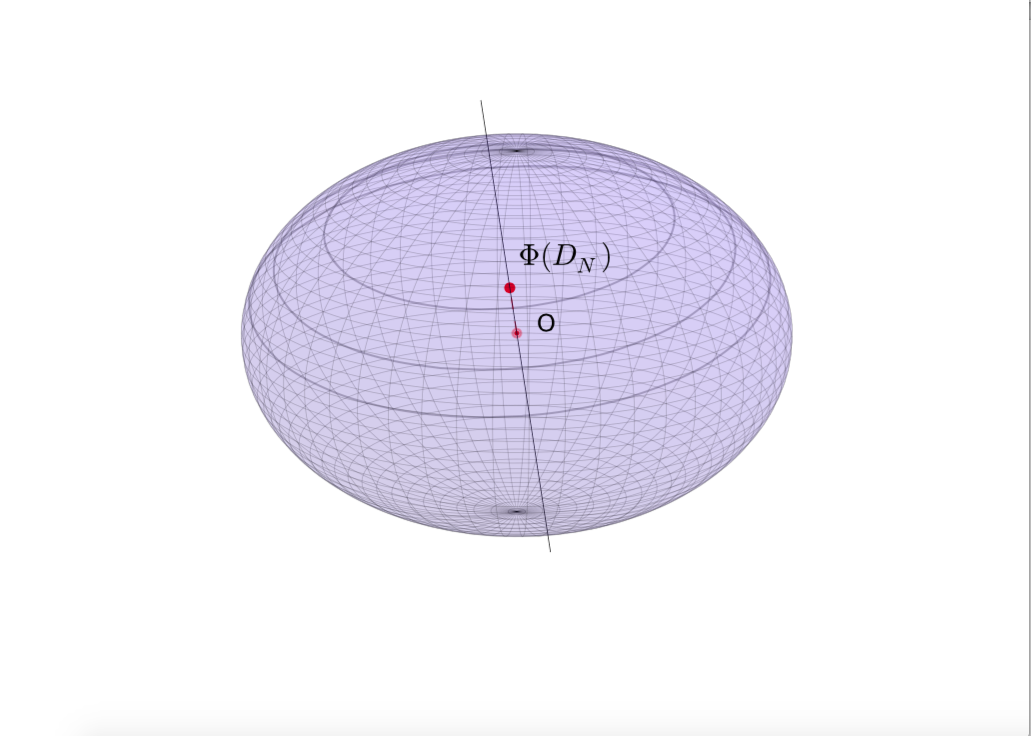
\includegraphics[trim=2cm 6cm 1cm 4cm, clip=true,  width=0.6\textwidth, height=2in]{ch-kemeny/figures/3d2test}
	\end{center}
	\caption{Level sets of the extended cost function $\CN$ over $\Sphere$ for $n=3$.}
	\label{figA:level-sets}
\end{figure}

\subsection{Interpretation of the Condition in Theorem \ref{thmA:method}}

The second element of our approach is motivated by the following observation. Let $x\in\Sphere$ be a point on the sphere and let $r \geq 0$. If $r$ is large enough, then all the points $x'\in\Sphere$ on the sphere that have distance $\nm{x'-x}$ greater than $r$ will have a greater angle $\theta_{N}(x')$. Formally, we denote by $\mathcal{B}(x,r) = \{x'\in\RR^{\binom{n}{2}} \;\vert\; \nm{x'-x} < r\}$ the (open) ball of center $x$ and radius $r$. Then one has the following result.

\begin{lemma}
\label{lemA:condition}
For $x\in\Sphere$ and $r\geq 0$, one has the following implication:
\[
\cos(\theta_{N}(x)) > \sqrt{1 - \frac{r^{2}}{4R^{2}}} \; \Longrightarrow \min_{x'\in\Sphere\setminus \mathcal{B}(x,r)}\theta_{N}(x') > \theta_{N}(x) \,.
\]
\end{lemma}

\begin{proof}
Let $\bar{\phi}(\DN) = \frac{\phi(\DN)}{\nm{\phi(\DN)}}$. We discuss over two cases.

\noindent {\bf Case I:} $\nm{\bar{\phi}(\DN) - x} \geq r.$ By laws of cosines, this case is equivalent to:
\begin{multline*}
2 R^2 (1-\cos(\theta_N(x))) = \nm{\bar{\phi}(\DN)  - x}^2 \geq r^2  \\
\Longleftrightarrow \cos(\theta_N(x)) \leq 1-\frac{r^2}{2R^2} \leq 1 -\frac{r^2}{4R^2} \,.
\end{multline*}
Note also that in this case, we have $\bar{\phi}(\DN)  \in \Sphere\setminus \mathcal{B}(x,r)$ and hence $\min_{x'\in\Sphere\setminus \mathcal{B}(x,r)}\theta_{N}(x') = \min_{x'\in\Sphere}\theta_{N}(x') = 0 \leq \theta_N(x)$ always holds, where the minimum is attained at $x'=\bar{\phi}(\DN)$.

\noindent {\bf Case II:} $\Vert\bar{\phi}(\DN)  - x\Vert < r$, that is $\bar{\phi}(\DN)  \in \mathcal{B}(x,r)$. As the function $x'\mapsto\theta_{N}(x')$ is convex with global minimum in $\mathcal{B}(x,r)$, its minimum over $\Sphere\setminus \mathcal{B}(x,r)$ is attained at the boundary $\Sphere \cap \partial \mathcal{B}(x,r) = \{x'\in\RR^{{n \choose 2}} \;\vert\; \nm{x'} = R \text{ and } \nm{x'-x} = r \}$, which is formed by cutting $\Sphere$ with the $\br{{n \choose 2}-1}$-dimensional hyperplane written as
$$
\mathbb{L} := \Big\{ x'\in\RR^{{n \choose 2}}\;\Big\vert\;\innerprod{x',x} = \frac{2R^2-r^2}{2}\Big\} \,.
$$
Straightforwardly one can verify that $\Sphere \cap \partial \mathcal{B}(x,r)$ is in fact a $\br{{n \choose 2}-1}$-dimensional sphere lying in $\mathbb{L}$, centered at $c = \frac{2R^2-r^2}{2R^2} x$ with radius $\gamma = r \sqrt{1-\frac{r^2}{4R^2}} \,.$ Now we take effort to identify:
$$
x^* = \argmin_{x' \in \Sphere \cap \partial \mathcal{B}(x,r)} \theta_N(x') = \argmin_{x' \in \Sphere \cap \partial \mathcal{B}(x,r)} \CN(x') \,.
$$
Note that $\phi(\DN)$ projected onto $\mathbb{L}$ is the vector $(\phi(\DN))_{\mathbb{L}} := \phi(\DN) - \frac{\innerprod{\phi(\DN),x}}{R^2}x.$ One can easily verify by Pythagoras rule that, for any set $\mathbb{K}\subseteq\mathbb{L}$,
$$
\argmin_{x'\in\mathbb{K}} \nm{x'-\phi(\DN)} = \argmin_{x'\in\mathbb{K}} \nm{x'-(\phi(\DN))_\mathbb{L}} \,.
$$
Therefore we have:
\begin{multline*}
x^* = \argmin_{x' \in \Sphere \cap \partial \mathcal{B}(x,r)} \nm{x'-(\phi(\DN))_\mathbb{L}} = c + \gamma \frac{(\phi(\DN))_\mathbb{L}}{\nm{(\phi(\DN))_\mathbb{L}}} \\
= \frac{2R^2-r^2}{2R^2} x + r \sqrt{1-\frac{r^2}{4R^2}} \frac{\phi(\DN) - \frac{\innerprod{\phi(\DN),x}}{R^2}x}{\sqrt{\nm{\phi(\DN)}^2 - \frac{\innerprod{\phi(\DN),x}^2}{R^2}}}\,.
\end{multline*}
Tedious but undemanding calculation leads to
\begin{equation*}
\theta_{N}(x^*) > \theta_{N}(x) \Longleftrightarrow \innerprod{x^*, \phi(\DN)} > \innerprod{x, \phi(\DN)} \Longleftrightarrow \cos(\theta_{N}(x)) > \sqrt{1 - \frac{r^{2}}{4R^{2}}} \,.
\end{equation*}
\end{proof}

It is interesting to look at the geometric interpretation of Lemma \ref{lemA:condition}. In fact, it is clear from the proof that $x^*$ should lie in the 2-dimensional subspace spanned by $\phi(\DN)$ and $x$. We are thus able to properly define multiples of an angle by summation of angles on such linear space $2\theta_N(x) := \theta_N(x) + \theta_N(x)$. Figure \ref{figA:illustration-condition} provides an illustration of Lemma \ref{lemA:condition} in this 2-dimensional subspace from the geometric point of view. In words, provided that $\theta_N(x)\leq \pi/2$, $x^*$ has a smaller angle than $x$ is equivalently written using laws of cosines as
\begin{multline*}
r^2 = \nm{x - x^*}^2 > 2 R^2 \big(1-\cos(2\theta_N(x))\big) \\
\Longleftrightarrow \cos(2\theta_N(x)) > 1 - \frac{r^2}{2R^2}
\Longleftrightarrow \cos(\theta_{N}(x)) > \sqrt{1 - \frac{r^{2}}{4R^{2}}} \,.
\end{multline*}
This recovers exactly the condition stated in Lemma \ref{lemA:condition}.

\begin{figure}[!htbp]
\begin{center}
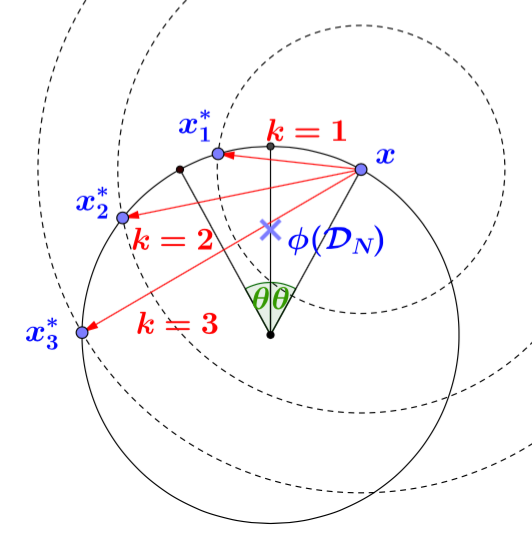
\includegraphics[width=0.6\textwidth]{ch-kemeny/figures/geomproof_big_r2k}
\end{center}
\caption{Geometric illustration of the bound in Lemma \ref{lemA:condition} with $x = \phi(\sigma)$ and $k=\frac{r^2}{4}$ taking integer values (representing possible Kendall's tau distance). The smallest integer value for $k$ such that these inequalities hold is $k=2$.}
\label{figA:illustration-condition}
\end{figure}


\subsection{Embedding of a Ball}

For $\sigma\in\Sn$ and $k\in\{0,\dots,\binom{n}{2}\}$ we denote by $B(\sigma,k)$ the (closed) ball for the Kendall's tau distance of center $\sigma$ and radius $k$, i.e. $B(\sigma,k) = \{\sigma'\in\Sn \;\vert\; d(\sigma,\sigma')\leq k\}$. The following is a direct consequence of Proposition \ref{propA:background-result}.

\begin{lemma}
\label{lemA:ball-embedding}
For $\sigma\in\Sn$ and $k\in\{0,\dots,\binom{n}{2}\}$,
\[
\phi\left( \Sn\setminus B(\sigma,k)\right) \; \subset \; \Sphere\setminus\mathcal{B}(\phi(\sigma),2\sqrt{k+1}) \,.
\]
\end{lemma}

\subsection{Proof of Theorem \ref{thmA:method}}

We can now prove Theorem \ref{thmA:method} by combining the previous results and observations.

\begin{proof}[Proof of Theorem \ref{thmA:method}]
Let $\DN\in\Sn^{N}$ be a dataset and $\sigma\in\Sn$ a permutation. By Lemma \ref{lemA:condition}, one has for any $r > 0$,
\begin{equation*}
\cos(\theta_{N}(\sigma)) > \sqrt{1 - \frac{r^{2}}{4R^{2}}} \Longrightarrow \min_{x\in\Sphere\setminus B(\phi(\sigma),r)}\theta_{N}(x) > \theta_{N}(\sigma) \,.
\end{equation*}
We take $r = 2\sqrt{k+1}$. The left-hand term becomes $\cos(\theta_{N}(\sigma)) > \sqrt{1 - \frac{k+1}{R^{2}}}$, which is the condition in Theorem \ref{thmA:method}. The right-hand term becomes:
\[
\min_{x\in\Sphere\setminus B(\phi(\sigma),2\sqrt{k+1})}\theta_{N}(x) > \theta_{N}(\sigma) \,,
\]
which implies by Lemma \ref{lemA:ball-embedding} that
\[
\min_{\sigma'\in\Sn\setminus B(\sigma,k)}\theta_{N}(\sigma') > \theta_{N}(\sigma) \,.
\]
This means that for all $\sigma'\in\Sn$ with $d(\sigma,\sigma') > k$, $\theta_{N}(\sigma') > \theta_{N}(\sigma)$. Now, by Lemma \ref{lemA:angles}, any Kemeny consensus $\sigstar$ necessarily satisfies $\theta_{N}(\sigstar) \leq \theta_{N}(\sigma)$. One therefore has $d(\sigma,\sigstar) \leq k$, and the proof is concluded.
\end{proof}



\section{Numerical Experiments}
\label{secA:experiments}


\subsection{Examples of Voting Rules}
\label{secA:votingrules}

In this section we study the tightness of the bound in Theorem \ref{thmA:method} and the applicability of The Method through numerical experiments. We first elaborate in detail the voting rules used in the chapter to approximate Kemeny's rule. Note that if multiple consensuses are returned from a rule on a given dataset, we always randomly pick one from these consensuses.

\begin{bulletList}
\item {\bf Positional scoring rules}. Given a scoring vector $w = (w_1,...,w_n) \in \RR^n$ of weights respectively for each alternative in $\n$, the $i$th alternative in a vote scores $w_i$. A total ranking is given by sorting the averaged scores over all votes, for example, the winner is the alternative with highest total score over all the votes. The \textbf{plurality} rule has the weight vector $(1,0,...,0)$, the \textbf{$k$-approval} rule has $(1,...,1,0...,0)$ containing 1s in the first $k$ positions, and the \textbf{Borda} rule \cite{Borda1781Memoire} has $(n, n-1, . . . , 1)$.
\item {\bf Copeland} \cite{Copeland1951reasonable}. A total ranking is given by sorting the Copeland scores averaged over all votes, for which the score of alternative $i$ is the number of pairwise beats, or $\#\{j \neq i: i \mbox{ beats } j\}$. For example, the Copeland winner is the alternative that wins the most pairwise elections.
\item {\bf QuickSort} \cite{Ali2012Experiments}. QuickSort recursively divides an unsorted list into two lists -- one list comprising alternatives that occur before a chosen index (called the \textit{pivot}), and another comprising alternatives that occur after, and then sorts each of the two lists. The pivot is always chosen as the first alternative.
\item {\bf Pick-a-Perm} \cite{Ali2012Experiments}. A total ranking is picked randomly from $\Sn$ according to the empirical distribution of the dataset $\DN$.
\item {\bf Plackett-Luce}. A Plackett-Luce ranking model defined for any $\sigma\in\Sn$ by $p_w(\sigma) = \prod_{i=1}^n w_{\sigma(i)}/\br{\sum_{j=i}^n w_{\sigma(j)}}$ parameterized by $w = (w_1,\dots,w_n)\in\RR^n$, fitted to $\DN$ by means of the MM algorithm \cite{Hunter2004MM}. A total ranking is then given by sorting $w$.
\item {\bf Pick-a-Random}. A total ranking is picked randomly from $\Sn$ according to uniform law (independent from $\DN$).
\end{bulletList}


Notably, Pick-a-Random is expected as a negative control experiment. To intuitively understand the rationale behind Pick-a-Random, let us consider the case conditioned on that the output of a voting rule has (at least) certain Kendall's tau distance to the Kemeny consensus. Compared to what Pick-a-Random would blindly pick any permutation without accessing to the dataset $\DN$ at all, a sensible voting rule should have a better chance to output one permutation with a smaller angle $\theta$ with $\phi(\DN)$ among all the permutations that share the same distance to Kemeny consensus. As we have reasoned in the geometric proof of The Method that the smaller the angle $\theta$ is, the more applicable our method will be, Pick-a-Random is expected to perform worse than other voting rules in terms of applicability of our method.



\subsection{Tightness of the Bound}

Recall that we denote by $n$ the number of alternatives, by $\DN\in\Sn^N$ any dataset, by $r$ any voting rule, and by $r(\DN)$ a consensus of $\DN$ given by $r$. For ease of notation convenience, we assume that $\KN$ contains a single consensus (otherwise we pick one randomly as we do in all experiments). The approximation efficiency of $r$ to Kemeny's rule is exactly measured by $d(r(\DN),\KN)$. Applying our method with $r(\DN)$ would return an upper bound for $d(r(\DN),\KN)$, that is: 
$$
d(r(\DN),\KN) \leq \kmin \,.
$$
Notably here we are not interested in studying the approximation efficiency of a particular voting rule, but we are rather interested in studying the approximation efficiency specific to our method indicated by the tightness of the bound, i.e.,
$$
s \br{r,\DN,n} := \kmin - d(r(\DN), \KN) \,.
$$
In other words, $s \br{r,\DN,n}$ quantifies how confident we are when we use $\kmin$ to ``approximate'' the approximation efficiency $d(r(\DN), \KN)$ of $r$ to Kemeny's rule on a given dataset $\DN$. The smaller $s \br{r,\DN,n}$ is, the better our method works when it is combined with the voting rule $r$ to pinpoint the Kemeny consensus on a given dataset $\DN$. Note that our notation stresses on the fact that $s$ depends typically on $\br{r,\DN,n}$. 


We empirically investigate the efficiency of our proposed method by experimenting $s \br{r,\DN,n}$ with various voting rules $r$, on different datasets $\DN$, implicitly involving $n$ as well. For that purpose, in each experiment we test six prevalent voting rules plus one negative-control method as approximate candidates to Kemeny's rule: three scoring rules that are Borda Count, $k$-approval, Copeland; two algorithmic approaches that are QuickSort and Pick-a-Perm; one statistical approach based on Plackett-Luce ranking model; one baseline method serving a negative control that is Pick-a-Random.


We first look at the the effect of different voting rules $r$ on $s \br{r;\DN,n}$ with the APA dataset. In the 1980 American Psychological Association (APA) presidential election, voters were asked to rank $n=5$ candidates in order of preference and a total of $N=5738$ complete ballots were reported. With the original collection of ballots introduced by \cite{Diaconis1989generalization}, We created $500$ bootstrapped pseudo-samples following \cite{Popova2012robust}. As shown in Figure \ref{figA:APA}, $s \br{r;\DN,n}$ varies across different voting rules and our method works typically well combined with Borda Count or Plackett-Luce, a phenomenon that constantly occurs in many experiments. For example for Borda Count the median tightness being $3$ means that our method provides a bound that tolerates an approximation within a Kendall's tau distance up to $3$. We also observe that on the contrary, the boxplot of Pick-a-Random always shows a wider range and larger median as expected. 


\begin{figure}[!htbp]
\begin{center}
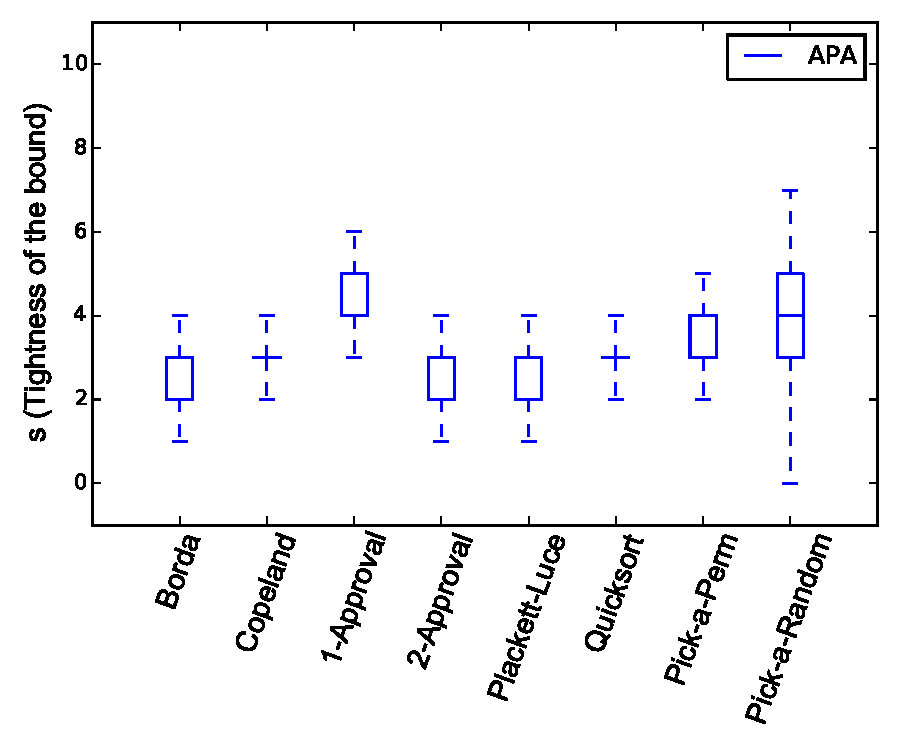
\includegraphics[width=0.6\textwidth]{ch-kemeny/experiments/APA.pdf}
\end{center}
\caption{Boxplots of $s \br{r,\DN,n}$ over sampling collections of datasets shows the effect from different voting rules $r$ with $500$ bootstrapped pseudo-samples of the APA dataset $(n=5,N=5738)$.}
\label{figA:APA}
\end{figure}


The effect of datasets $\DN$ on the measure $s \br{\DN;r,n}$ is tested with the Netflix data provided by \cite{Mattei2012empirical}. We set $n=3$ the number of ranked alternatives and take two types of data with distinct characteristics to contrast their impact: we took the $100$ datasets with a Condorcet winner and randomly selected $100$ datasets from those with no Condorcet winner. The rationale for this experiment is that Kemeny's rule is a Condorcet method, i.e., Kemeny's rule always yields a Condorcet winner if it exists. Therefore we suppose that the efficiency of our method should also depend on this particular social characteristic present in data. As expected, it is interesting to note the clear difference shown by the two types of data shown by Figure \ref{figA:netflix}. In words, our method is more efficient in case that a Condorcet winner is present in the dataset than the other case that a Condorcet winner is absent in the sense that $s$ is generally smaller in the former case.


\begin{figure}[!htbp]
\begin{center}
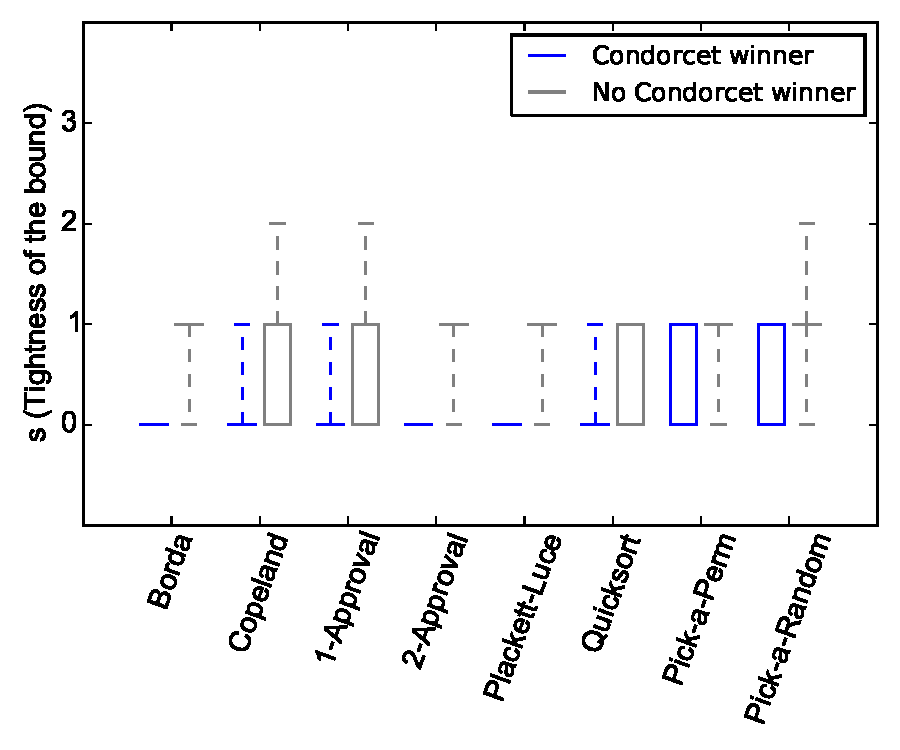
\includegraphics[width=0.6\textwidth]{ch-kemeny/experiments/netflix.pdf}
\end{center}
\caption{Boxplots of $s \br{r,\DN,n}$ over sampling collections of datasets shows the effect from datasets $\DN$. $100$ Netflix datasets with the presence of Condorcet winner and $100$ datasets with no Condorcet winner ($n=4$ and $N$ varies for each sample).}
\label{figA:netflix}
\end{figure}


We finally study how the $s \br{n;r,\DN}$ grows with the size of the alternative set $n$ using the sushi dataset found in \cite{Kamishima2003Nantonac}, originally provided as a dataset of $N=5000$ total rankings of $10$ sushi dishes. As evaluating $s$ requires exact Kemeny consensus which can quickly become intractable when $n$ is large, we strict in this study the number of sushi dishes $n$ to be relatively small, and generate collections of datasets, indexed by combinations of $n$ sushi dishes out of $\cbr{1,\dots,10}$, by counting the total occurrences of such order present in the original dataset. For example, when $n=3$ we have a total of ${10 \choose 3} = 120$ different combinations of alternatives (hence $120$ collections of datasets) each generated by counting the total occurrences of preference orders of individuals restricted to these $3$ alternatives. Therefore we have a total of $120;210;252$ datasets respectively for $n=3;4;5$. Figure \ref{figA:sushi} shows that $s \br{r,\DN,n}$ increases as $n$ grows, a trend that is dominant and consistent across all voting rules. Since the maximal distance ${n \choose 2}$ in $\Sn$ grows quadratically with respect to $n$, an interesting question would remain to specify explicitly the dependency of $\kmin$ on $n$, or the dependency of $s\br{r,\DN,n}$ on $n$, for a given voting rule.


\begin{figure}[!htbp]
\begin{center}
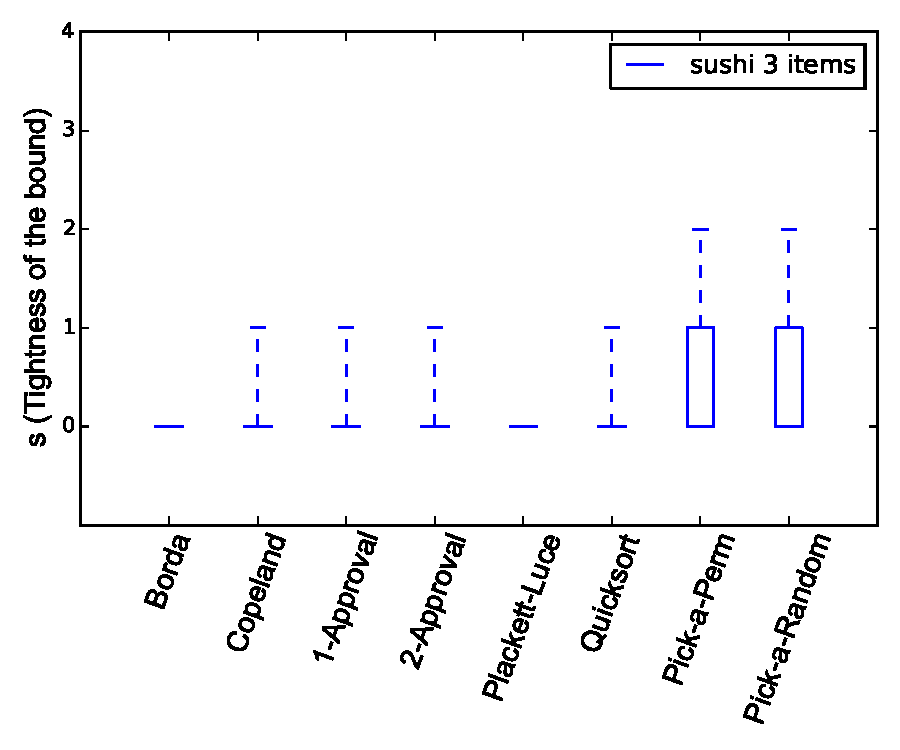
\includegraphics[width=0.3\textwidth]{ch-kemeny/experiments/sushi3.pdf}
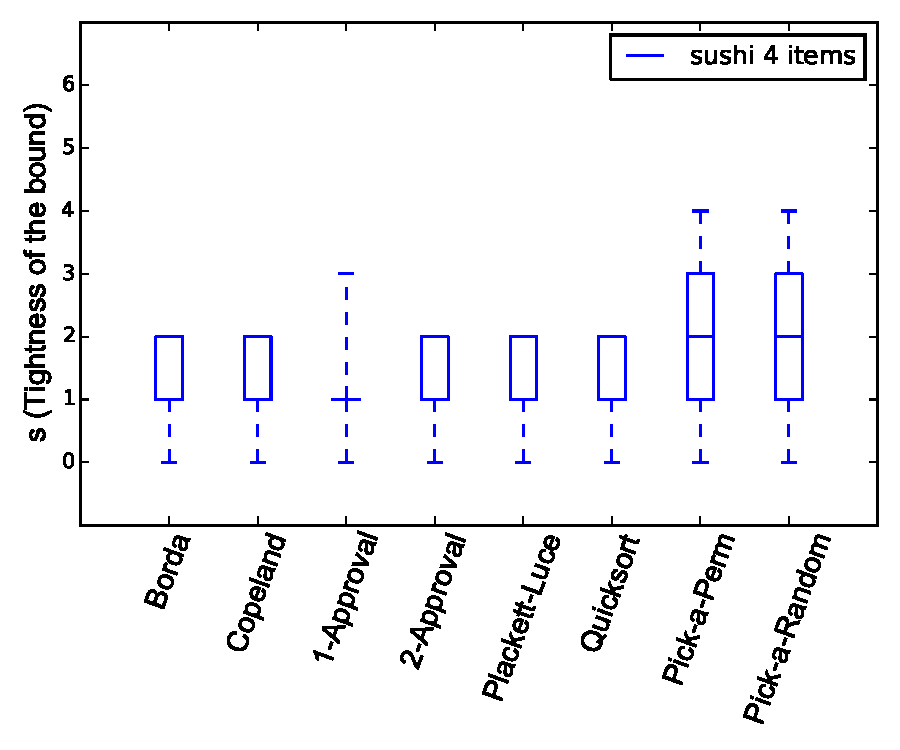
\includegraphics[width=0.3\textwidth]{ch-kemeny/experiments/sushi4.pdf}
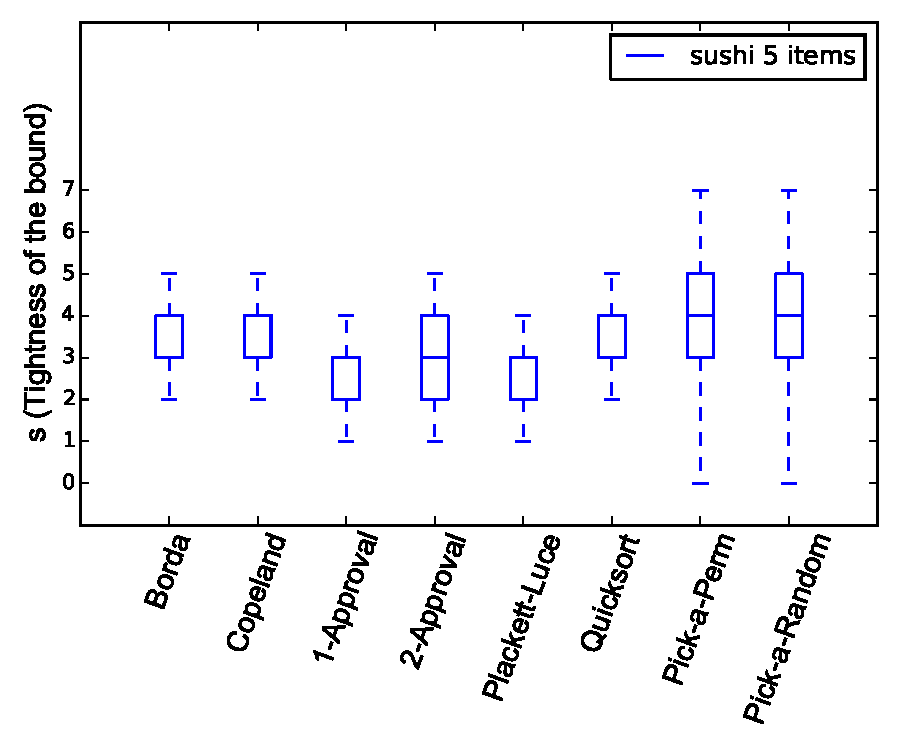
\includegraphics[width=0.3\textwidth]{ch-kemeny/experiments/sushi5.pdf}
\end{center}
\caption{Boxplots of $s \br{r,\DN,n}$ over sampling collections of datasets shows the effect from different size of alternative set $n$ with restricted sushi datasets $(n=3;4;5,N=5000)$.}
\label{figA:sushi}
\end{figure}




\subsection{Applicability of The Method} 

We have so far focused on small $n$ $(n \leq 5)$ case, and verified that our method is efficient in using $\kmin$ to approximate $d(r(\DN),\KN)$. We are now mostly interested in the usefulness of our method when $\kmin$ is directly combined with voting rules in pinpointing Kemeny consensus $\KN$ particularly when $n$ is large. Now we employ our method by using $\kmin$ for each dataset to upper bound the approximation performance of $r(\DN)$ to Kemeny's rule. Moreover, suppose that we are still interested in finding the exact Kemeny consensus despite a good approximation $r(\DN)$. Once we have computed an approximated ranking $r(\DN)$ and $\kmin$ is identified via our method, the search scope for the exact Kemeny consensuses can be narrowed down to those permutations within a distance of $\kmin$ to $r(\DN)$. Notably \cite[Lemma 1]{Wang2013rate} proved that the total number of such permutations in $\Sn$ is upper bounded by ${n + \kmin -1 \choose \kmin}$ which can be smaller than $\abs{\Sn} = n!$ by orders.



We took the original sushi dataset consisting of $N=5000$ individual votes on $n=10$ sushi dishes and created $500$ bootstrapped pseudo-samples following the same empirical distribution. Note that $\kmin$ should also depend on $\br{r,\DN,n}$. Since our bound is established in general with any $\sigma\in\Sn$ and does take into consideration the approximation efficiency of specific voting rules to Kemeny's rule, the predicted $\kmin$ should significantly rely on the approximate voting rules utilized and should be biased more in favor to voting rules with good approximation to Kemeny's rule since $\kmin$ can never be inferior to $d(r(\DN),\KN)$. As shown in Figure \ref{figA:applicability}, Pick-a-Random and Pick-a-Perm typically performs poorly, but this is largely due to the fact that the two voting rules are too naive to well approximate Kemeny's rule \textit{per se}. On the contrary, we observe that Borda, Copeland and QuickSort combined with our method best pinpoint Kemeny consensuses with $\kmin$ of a median distance $14$. This further means that in order to obtain all the exact Kemeny consensuses now, on average we need to search through at most ${10 + 14 -1 \choose 14} = 817,190$ permutations instead of $10! = 3,628,800$ permutations, where 77\% of permutations in $\mathbb{S}_{10}$ are removed from consideration.


\begin{figure}[!htbp]
\begin{center}
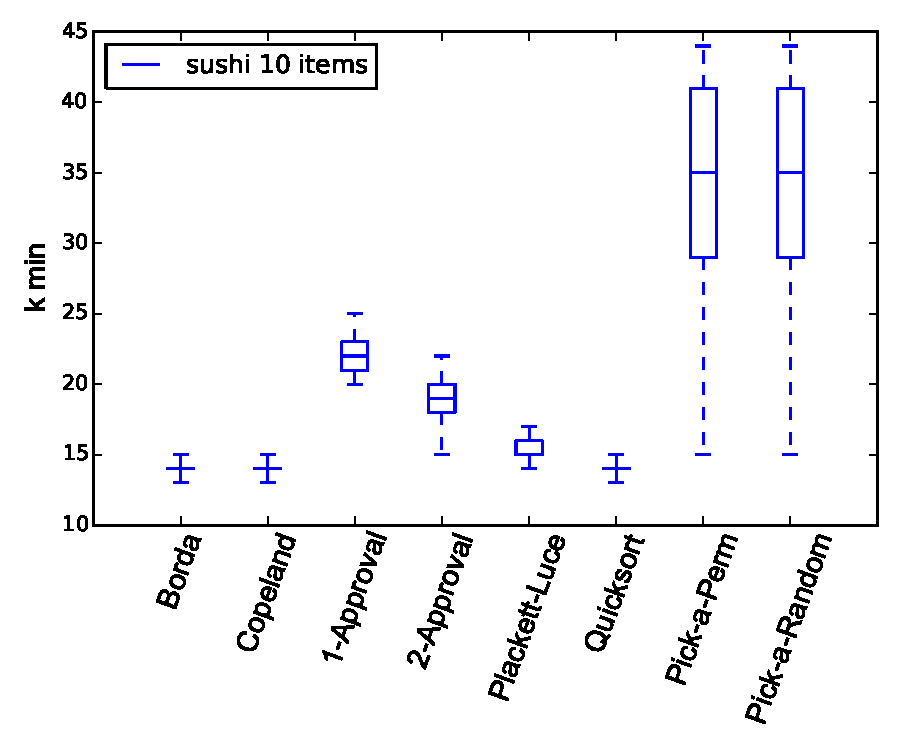
\includegraphics[width=0.6\textwidth]{ch-kemeny/experiments/sushi10.pdf}
\end{center}
\caption{Boxplots of $\kmin$ over $500$ bootstrapped pseudo-samples of the sushi dataset $(n=10, N=5000)$.}
\label{figA:applicability}
\end{figure}



\section{Discussion}

In this chapter, we have established a theoretical result that allows to control the Kendall's tau distance between a permutation and the Kemeny consensuses of any dataset. In practice, this provides a simple and general method to predict, for any ranking aggregation procedure, how close its output on a dataset is from the Kemeny consensuses. From a broader perspective, it constitutes a novel approach to apprehend the complexity of Kemeny aggregation.

Our results rely on the geometric properties of the Kendall embedding. Though it has rarely been used in the literature, it provides a powerful framework to analyze Kemeny aggregation. We therefore believe that it could pave way to other profound results. In particular, we deem that an analysis of how the embeddings of the permutation spread on the sphere could lead to a finer condition in Theorem \ref{thmA:method}, which is left as future work.

Another interesting direction would certainly be to extend our method to rank aggregation from partial orders, such as pairwise comparisons or top-$k$ rankings. Two main approaches can be followed. In the first one, a partial order would be identified with the set $S\subset\Sn$ of its linear extensions and its distance to a permutation $\sigma\in\Sn$ defined by the average $(1/\vert S\vert)\sum_{\sigma'\in S}d(\sigma,\sigma')$. The Kendall embedding would then naturally be extended to $S$ as $(1/\vert S\vert)\sum_{\sigma'\in S}\phi(\sigma')$, the barycenter of embeddings of its linear extensions. In the second approach, one would see a partial order as a collection of pairwise comparisons $\{i_{1}\succ j_{1}, \dots, i_{m}\succ j_{m}\}$ and define its distance to a permutation $\sigma\in\Sn$ by the average number of pairwise disagreements $(1/m)\sum_{r=1}^{m}\hollowone\{\sigma(i_{r}) > \sigma(j_{r})\}$. The Kendall embedding would then naturally be extended to $\{i_{1}\succ j_{1}, \dots, i_{m}\succ j_{m}\}$ as the embedding of any linear extension $\sigma$ where the coordinate on $\{i,j\}$ is put equal to $0$ if $\{i,j\}$ does not appear in the collection. In both cases, our approach would apply with slight changes to exploit related geometric properties.
